% Frame: Reasoning Example (step-by-step, with answer highlighted)
\begin{frame}{Reasoning}
  \centering
  % Main diagram box (rounded rectangle with blue border)
  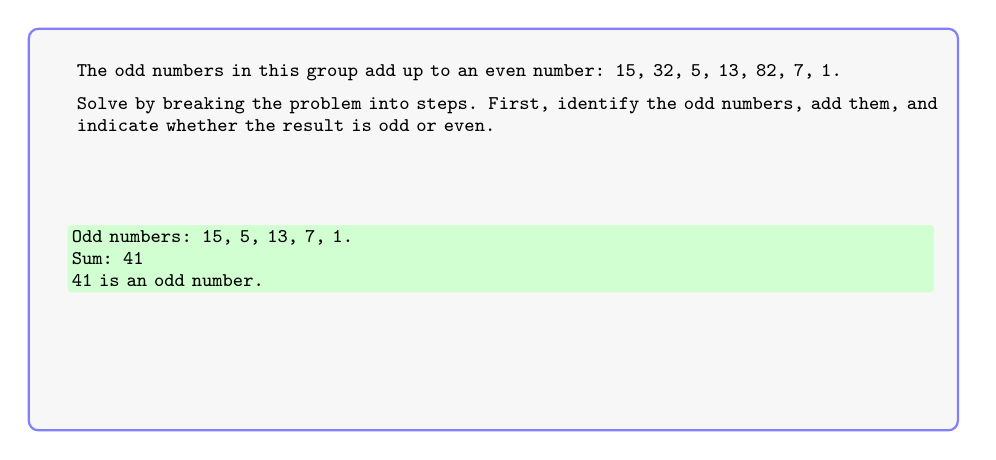
\begin{tikzpicture}
    % Outer box
    \node[fill=gray!6, draw=blue!50, thick, rounded corners=3.5pt, minimum width=11.8cm, minimum height=5.1cm, anchor=north west, inner sep=0pt] (mainbox) at (0,5.3) {};

    % Problem statement (monospaced, gray text)
    \node[anchor=north west, font=\ttfamily\scriptsize, align=left, text width=11.2cm] (context) at ([xshift=0.5cm, yshift=-0.35cm]mainbox.north west) {%
The odd numbers in this group add up to an even number: 15, 32, 5, 13, 82, 7, 1.\\[.5em]
Solve by breaking the problem into steps. First, identify the odd numbers, add them, and indicate whether the result is odd or even.
    };

    % Reasoning steps (highlighted in green background)
    \node[anchor=north west, font=\ttfamily\scriptsize, fill=green!18, rounded corners=1.3pt, text width=10.9cm, inner xsep=1.5pt, inner ysep=2.0pt, yshift=-2.5cm] (steps) at ([xshift=0.5cm]mainbox.north west) {%
\textcolor{black}{Odd numbers: 15, 5, 13, 7, 1.}\\
\textcolor{black}{Sum: 41}\\
\textcolor{black}{41 is an odd number.}
    };

  \end{tikzpicture}
\end{frame}
